\chapter{Characterisation of the optical setup}

\textit{In the previous chapter we seeked for different aspects of the
\gls{rf} signal powering the \gls{aod} elements and found that the
electronic equipement provides an overall stable signal for the \gls{aod}.
In this chapter we want to examine the intensity characteristics subject
to frequency and amplitude parameters of the \gls{rf} signal. In the end
we will find that the intensity shows highly non-linear behaviour with
respect to the \gls{rf} signal parameters.}

\section{Intensity control}

As already stated in the experimental setup \cref{ch:experimental_setup} the
laser intensity is regulated by a control loop using an \gls{aom} in the
power reduction setup. Without the additional intensity regulation we would
observe various intensity drifts from the laser source throughout the
measurements. To ensure that the laser intensity is stable, and to estimate
the error contribution of an imperfect intensity, we will conduct a short-term
and a long-term measurement of the controlled intensity. In fact a typical
intensity measurement takes about a fraction of a millisecond, yet we can
decide on different intervals between the measurements in order to separate
local from global trends. \Cref{tab:intensity_control_times} summarizes the
different time intervals for the conducted short- and long-term measurement
of the intensity control and a measurement involving the \gls{aod}s.
\begin{table}[h]
  \centering
  \begin{tabular}{|c|c|c|c|c|c|}
    \hline
    & Short & Long & Sweep \\
    \hline
    Interval &
    \SI{10}{\second} &
    \SI{120}{\second} &
    \SI{3}{\second} \\
    \hline
    Duration &
    \SI{1}{\hour} &
    \SI{16}{\hour} &
    \SI{<2}{\hour} \\
    \hline
  \end{tabular}
  \captionsetup{width=.8\textwidth}
  \caption{Interval and duration times of the short- and long-term measurement
    as well as a typical sweep measurement discussed in later sections.
  }\label{tab:intensity_control_times}
\end{table}
The experimental setup is the same as described in
\cref{ch:experimental_setup}, however we disassembled the \gls{aod} and placed
Photodiode 2 at the end of the laser beam. The setup is depicted in
\Cref{fig:intensity_control_setup}. The photodiode gain of Photodiode 2 was
lowered from \SI{70}{\decibel} to \SI{50}{\decibel} because the absence of the
\gls{aod}s would otherwise cause the photodiode to saturate.
\begin{figure}[ht]
  \centering
  \includegraphics[width=.9\textwidth]{\mediadir{setup/intensity-control.pdf}}
  \captionsetup{width=.9\textwidth}
  \caption{Optical setup and intensity detection. The beam hits Photodiode 2
    which is connected to the oscilloscope.
  }\label{fig:intensity_control_setup}
\end{figure}
If not noted elsewise we will transform the voltages through
\begin{equation}
  U
  =U_0 10^{-\SI{20}{\decibel}/\SI{10}{\decibel}}
  =U_0 10^{-2}
  \label{eq:voltage_gain}.
\end{equation}
The voltage time series for both intensity control measurements are presented
in \Cref{fig:intensity_control}. The outlier at about 22:45 h was caused by
accidently interfering with the setup during measurement. Beside of that
incident the long-term intensity seems stable. For the short-term measurement
we observe small oscillations on the fine time scale.
\begin{figure}[ht]
  \centering
  \includegraphics[width=\textwidth]{\figuredir{intensity/control/long-short.pdf}}
  \captionsetup{width=.8\textwidth}
  \caption{Long- and short-term measurement of the controlled intensity. In
  the first row we compare the short-term measurement to the voltage scale
  of the long-term measurement. In the second row both plots use the voltage
  scale of the short-term measurement.
  }\label{fig:intensity_control}
\end{figure}
\Cref{tab:intensity_control} depicts the corresponding descriptive statistics
of the intensity voltage time series and an intensity measure involving the
\gls{aod}s for comparison.
\begin{table}[h]
  \centering
  \begin{tabular}{|c|c|c|c|c|c|}
    \hline
    & Long & Short & Sweep \\
    \hline
    Mean $\mu$ &
    \SI{6.79}{\volt} &
    \SI{6.79}{\volt} &
    \SI{1.95}{\volt} \\
    \hline
    Minimum &
    \SI{4.88}{\volt} &
    \SI{6.77}{\volt} &
    \SI{0.00}{\volt} \\
    \hline
    Maximum &
    \SI{6.86}{\volt} &
    \SI{6.82}{\volt} &
    \SI{3.00}{\volt} \\
    \hline
    Standard Deviation $\sigma$ &
    \SI{0.09}{\volt} &
    \SI{0.01}{\volt} &
    \SI{0.54}{\volt} \\
    \hline
    Relative Standard Deviation $\sigma/\mu$ &
    \SI{1.35}{\percent} &
    \SI{0.19}{\percent} &
    \SI{27.7}{\percent} \\
    \hline
  \end{tabular}
  \captionsetup{width=.8\textwidth}
  \caption{Descriptive statistics of the short term measurement of the
  intensity with controlled intensity. Note the small standard deviation.}
  \label{tab:intensity_control}
\end{table}

The previous section gave us already some good insights about the long term
stability of the intensity control loop. Yet in practice typical intensity
measurements are of much smaller magnitude, henceforth it seems close at hand
to also conduct a short term measurement.

For the short term measurement time parameters were adjusted to a sample
interval of \SI{10}{\second} and measurment were performed over \SI{1}{\hour}.

The intensity time series of the short term measurement is depicted in
\Cref{fig:intensity_control_short} and the associated descriptive
statistics are presented in \Cref{tab:intensity_control_short}.

On a smaller timescale we see that the intensity control loop performs
periodic oscillations, however the descriptive statistics show much smaller
deviation from the mean, than observed in the long term measurements. As we
do not see outliers in \Cref{fig:intensity_control_short} we can pay more
attention to the value range of \SI{0.05}{\volt} which was obfuscated in
the long term measurement because of outliers.

\subsubsection{Summary}

The previous discussion confirmed that the intensity is regulated in that
we only observe oscillations around the targeted intensity value. Yet we are
still missing statements with regard to the magnitude of these oscillations
as we are missing a comparison to real intensity data.

For a typical measurement, to compare the intensity oscillations with, we
elected the intensity progression of a linear frequency sweep of the
\gls{aod} in the vertical socket while the \gls{aod} in the horizontal socket
is fixed. We will discuss this specific meausurement in detail in a later
section. In \Cref{tab:intensity_control} we see some statistics of the
long and short term measurements next to the typical measurement.
\begin{figure}[ht]
  \centering
  \includegraphics[width=\textwidth]{\figuredir{intensity/control/deviation.pdf}}
  \captionsetup{width=.8\textwidth}
  \caption{Boxplot of the long and short term intensity measurements and a typical
  intensity measurement with the \gls{aod} where we subtracted the mean intensity
  for comparison. The typical measurements covers a much wider intensity range
then deviations from the intensity control loop.
  }\label{fig:intensity_control_comparison}
\end{figure}
One dismally error estimate would be the quotient of the value range of the
short term measurement and the typical measurement, yielding an error of
\SI{4.2}{\percent}. A second approach would be the quotient of the standard
deviation of the short term and typical measurement, yielding
\SI{2.5}{\percent} error. When comparing the typical measurement to the
statictis of a long term measurement we find rather large errors which
suggests that there re other statistical key figures which may be more
suitable.

A boxplot is very useful in visualizing the spread. We have an orange stripe
marking the median, the contour of the box marking the data between first and
third quantil. The usual value range is marked by the whiskers and outliers
are marked as the circles outside the whiskers.
In \Cref{fig:intensity_control_comparison} we see such a boxplot for the
absolute deviation from the mean of the three measurements. The absolute
deviation from the mean accounts for the different transmission just because
of the presence of the \gls{aod} in the typical measurement but keeps the
linear scale unlike the squared deviation from mean. We can see that in a
typical measurement (upper boxplot) the usual deviation from mean is much
larger than for the short and long term measurement of the intensity
regulation.

\section{Beam profile}

Perpendicular to the error introduced by the imperfect intensity control,
errors can originate from unideal optical alignment and calibration. One way
to assess the quality of our alignment is to evaluate the spatial profile of
the laser beam as registered with the \gls{ccd} camera.

In the previous setup we used a second photodiode to measure the temporal
deviations of the intensity. In order to measure spatial deviations of the
intensity we replaced the photodiode with a \gls{ccd} camera. In
\Cref{fig:intensity_profile_setup} we see the setup used to measure the beam
profile. The \gls{aod}s are configured at a center frequency of
\SI{100}{\mega\hertz}. The distance between Lens 4 and the \gls{ccd} sensor is
chosen such that the laser beam is focused onto the \gls{ccd} sensor of the
camera.
\begin{figure}[ht]
  \centering
  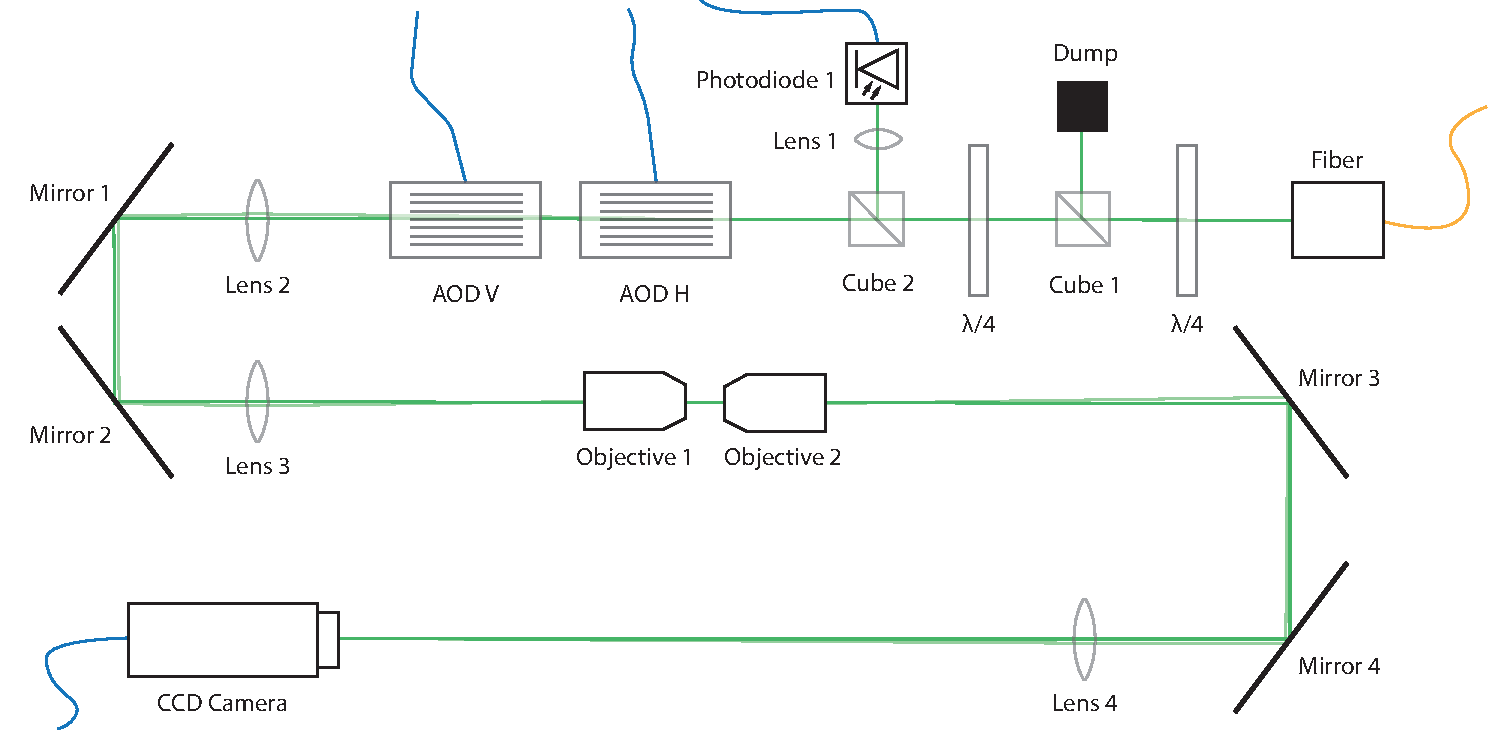
\includegraphics[width=\textwidth]{\mediadir{setup/intensity-profile.pdf}}
  \captionsetup{width=.8\textwidth}
  \caption{The beam is focused onto the \gls{ccd} sensor of the camera. The
    \gls{aod} are configured at \SI{100}{\mega\hertz} center frequency.
  }\label{fig:intensity_profile_setup}
\end{figure}
In \Cref{fig:intensity_profile_2d} we can see an enlarged image patch of the
complete image capture taken with the \gls{ccd} camera. We can see a strong
illuminated circular spot in the center of the image with an area of about
\SI{2.5}{\milli\meter}. The intensity inside the spot seems homogeneous,
however this is caused by a saturation of the pixels in this area. We could
reduce the intensity or apply an optical filter to the camera to resolve the
intensity gradient inside the spot, but only at the cost of the intensity
distribution around the spot. Around the circular spot we can see a
diffraction ring. The diffraction ring is well described in
\cite{Hertlein2017} and originates from the finite aperture of the objectives.
\begin{figure}[ht]
  \centering
  \includegraphics[width=.5\textwidth]{\figuredir{intensity/profile/profile2d.pdf}}
  \caption{Image of the focused laser beam measured with the \gls{ccd} camera.}
  \label{fig:intensity_profile_2d}
\end{figure}
For better comparison of the radial symmetry we performed two perpendicular
cuts and visualized the one dimensional spatial beam distribution in
\Cref{fig:intensity_profile_1d}.
\begin{figure}[ht]
  \centering
  \includegraphics[width=.9\textwidth]{\figuredir{intensity/profile/profile1d.pdf}}
  \captionsetup{width=.8\textwidth}
  \caption{One dimensional perpendicular cut of the two dimensional intensity
    distribution from the two dimensional beam profile in
    \Cref{fig:intensity_profile_2d} with fitted gaussian curve.}
  \label{fig:intensity_profile_1d}
\end{figure}
In \Cref{fig:intensity_profile_1d} we can clearly observe the effects of
saturation around the center and how we would expect the intensity to be
if we could experimentally resolve it in the Gaussian fit. In contrast to the
ideal Gaussian profile we again observe contributions to the Airy disc around
the otherwise Gaussian profile causes by the finite aperture. Further we can
now clearly observe assymmetry from the intensity contributions around the
Gaussian which means that our alignment is not perfect.

We can confirm the results reported in \cite{Hertlein2017} that the spatial
beam profile equals a two dimensional Gaussian combined with a Airy disks
caused from the finite aperture of the objectives. Further we observe
slight assymmetries in the diffraction ring suggesting inperfect alignment.
Though asymetries in the spatial beam profile are present, we do not see any
further complications as the intensity measurements with the photodiode will
cover the complete beam profile.

\section{Difference between individual acousto-optic deflectors}

Our optical setup uses a single two dimensional \gls{aod} that comprises two
\gls{aod} elements perpendicular to each other. At first we want to examine the
behaviour of the individual \gls{aod} elements to each other. In particular we
are interested if and how the elements differ.

A schematic drawing of the \gls{aod} is depicted in \Cref{fig:aod_socket}. We see the
two \gls{aod} elements in the respective horizontal and vertical slot. The
internals of the vertical \gls{aod} (left-hand side) are illustrated. The
element itself spans through the casing (dashed line) while the acousto-optic
crystal (dotted line) is glued onto the element. The laser beam (green) passes
through the acousto-optic crystal. In the following we will refer to the
horizontal \gls{aod} element as the \gls{aod} element anticipated for the
horizontal slot and accordingly to the vertical \gls{aod} element as the
\gls{aod} element intended for the vertical \gls{aod} socket.
\begin{figure}[ht]
  \centering
  \includegraphics[width=\textwidth]{\mediadir{setup/aod-socket.png}}
  \captionsetup{width=.8\textwidth}
  \caption{Drawing of the used 2D \gls{aod}. The 2D \gls{aod} comprises two
    perpendicular orientated \gls{aod} elements.
  }\label{fig:aod_socket}
\end{figure}

\subsection{Individual acousto-optic deflectors}

For the following experiment we will only leave one \gls{aod} element mounted
in the casing depicted in \Cref{fig:aod_socket}. The other slot will be empty.
Then we will exchange socket positions for each respective \gls{aod} element
and measure the beam intensity subject to the linear frequency sweep from
\SI{80}{\mega\hertz} to \SI{120}{\mega\hertz} over a duration of
\SI{260}{\milli\second} and the configured \gls{dds} amplitude. As \gls{rf}
signal source the amplifier and \gls{dds} combination intended for the
horizontal \gls{aod} element was used to avoid influences of the amplification
offset between the two amplifiers.

The results for the four configurations (horizontal element in horizontal slot,
horizontal element in vertical slot, vertical element in horizontal slot
and vertical element in vertical slot) are visualized as heatmaps in
\Cref{fig:intensity_distribution_unpaired}. The color values are normalized in between the
different heatmaps and can be related to the measured voltage from the
photodiode via the colorbar on the right-hand side.
\begin{figure}[ht]
  \centering
  \includegraphics[width=\textwidth]{\figuredir{intensity/distribution/unpaired-amplitude.png}}
  \captionsetup{width=.8\textwidth}
  \caption{Intensity distribution over linear frequency sweep at different
  configured \gls{dds} amplitudes for different individual \gls{aod}
  configurations.
  }\label{fig:intensity_distribution_unpaired}
\end{figure}
Oddly enough we observe that both \gls{aod}s differ strongly in their
respective intensity transmission behaviour depending on their slot position.
Furthermore we observe that the intensity transmission is much higher in the
case of the horizontal \gls{aod} element mounted to the intended horizontal
slot compared to all other configurations. In addition we can see that the
intensity map measured with the horizontal \gls{aod} displays a jump. The
highest intensity transmission is obtained for relative
amplitudes configured between \SI{60}{\percent} and \SI{90}{\percent} with
large dependence on the frequency. Another interesting observation is that
the intensity transmission seems very similar for the horizontal element in
the vertical slot and the vertical element in the vertical slot whose
map also seems more symmetric with respect to the frequency axis. In fact
for these configurations the amplitude dependence seems to be essentially
independent of the frequency dependence.

\subsection{Paired acousto-optic deflectors}

The \gls{aod} elements differ significantly in their intensity transmission
in between and with respect to their position. We find the horizontal element
in the anticipated horizontal position to have a significantly higher
transmission then any other configuration. Therefore we presume that the
\gls{aod} elements have a very high polarization dependency and are concerted
to eachother. We may find more evidence for this hypothesis by mounting both
\gls{aod} elements in their intended and exchanged slots.
\begin{figure}[ht]
  \centering
  \includegraphics[width=\textwidth]{\figuredir{intensity/distribution/paired-amplitude.png}}
  \captionsetup{width=.8\textwidth}
  \caption{Intensity distribution over linear frequency sweep at different
  configured \gls{dds} amplitudes for different individual \gls{aod}
  configurations.
  }\label{fig:intensity_distribution_paired}
\end{figure}
In \Cref{fig:intensity_distribution_paired} the measured voltage of the
second photodiode are visualized in a two-dimensional heatmap. The horizontal
axis represents the frequency of the \gls{rf} signal applied to the \gls{aod}
elements whereas the vertical axis the configured \gls{dds} relative
amplitude. In the first row the elements where in their intended slots whereas
we exchanged them for the second row. In the first column the frequency
sweep was applied such that the beam moves along the horizontal axis while
in the second column the frequency sweep was applied to the element that
causes beam movement in the vertical direction.

We see that for the exchanged positions the transmission is reduced and
asymmetric with respect to the sweep direction whereas the elements in their
intended position perform better in every aspect. We therefore conclude that
the \gls{aod} are cut in a intended way to account among others for
polarization effects and it is advised to operate them in their anticipated
slot as we will do for all following experiments.

\section{2D intensity distribution}

In the previous section we sorted out the influence of the \gls{aod} element
position and acknowledged that \gls{aod}s differ significant in their
optical properties. In the present section we now want to explore the
intensity transmission for a two dimensional sweep as intended to be used
for the optical potentials.

The experimental setup is similar to the previous setups and is shown in
\Cref{fig:intensity_distribution_setup}. We have both \gls{aod}s mounted in
their anticipated position. The \gls{aod} elements are aligned to maximize
intensity at the center frequency. The laser beam is directed into a second
photodiode where we measure the intensity with respect to the configured
\gls{dds} signal.
\begin{figure}[ht]
  \centering
  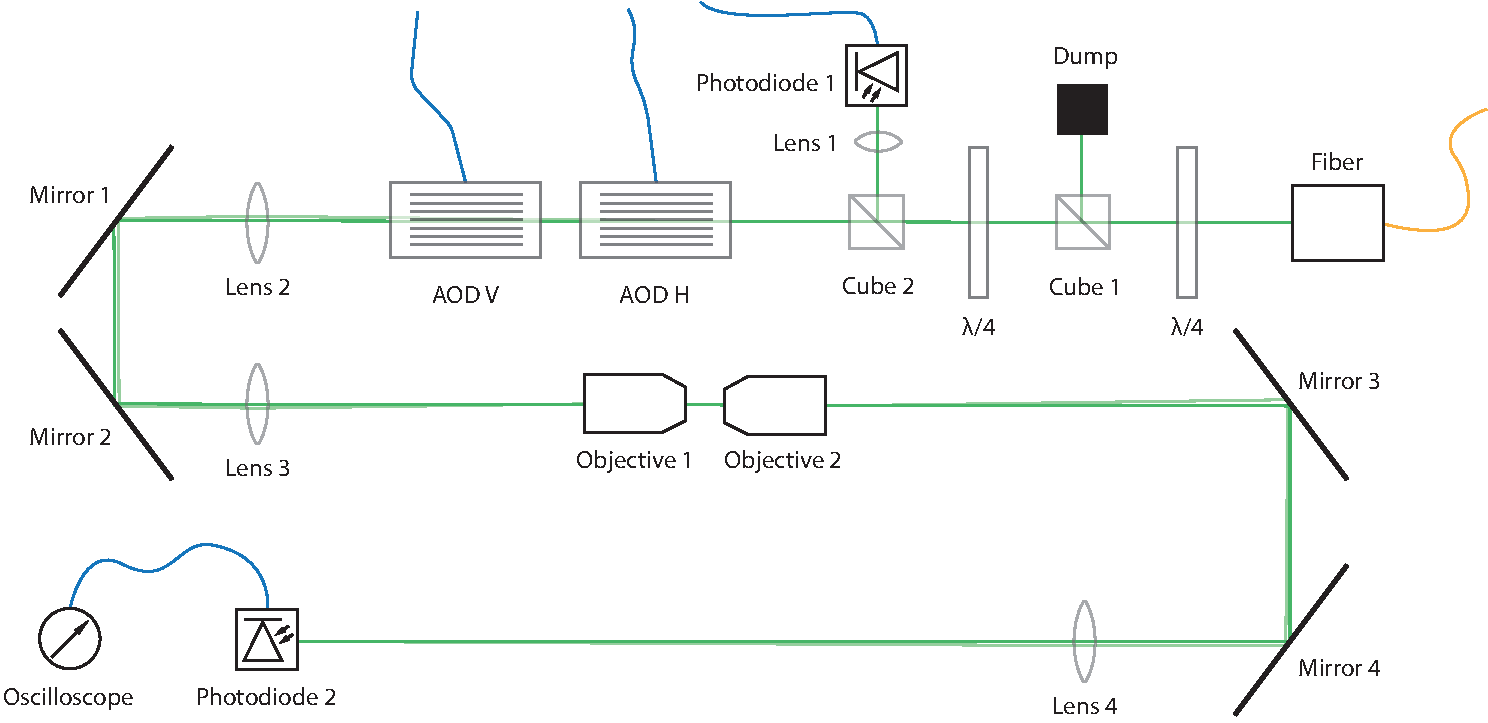
\includegraphics[width=\textwidth]{\mediadir{setup/intensity-distribution.pdf}}
  \captionsetup{width=.8\textwidth}
  \caption{Experimental setup used to measure the intensity transmission of
  the 2D \gls{aod} in dependence of the configured \gls{dds} signal.}
  \label{fig:intensity_distribution_setup}
\end{figure}

\subsubsection{Digital ramp frequency sweep}

In a first attempt we configure a first \gls{dds} to output a constant
frequency whereas a second \gls{dds} is configured to do a frequency sweep
using the internal digital ramp. After one such sweep the constant frequency
output of the first \gls{dds} is increased and the measurement repeats. The
procedure is repeated until the first \gls{dds} covered the same frequency
range as the second \gls{dds}.
\begin{figure}[ht]
  \centering
  \includegraphics[width=\textwidth]{\figuredir{intensity/distribution/paired-frequency.png}}
  \captionsetup{width=.8\textwidth}
  \caption{Intensity measured as voltage at the photodiode in dependence of
    the horizontal and vertical applied frequency signal to the \gls{aod}. The
    left map is obtained by enabling the digital ramp on the horizontal
    \gls{dds} whereas the vertical \gls{dds} is configured to output a
    constant frequency which is manually increased after each measurement.
    On the right-hand side map the roles are exchanged.}
  \label{fig:intensity_distribution_frequency}
\end{figure}
In \Cref{fig:intensity_distribution_frequency} we present the intensity
measured at the second photodiode in the setup shown in
\Cref{fig:intensity_distribution_setup}. On the left-hand map the first
\gls{dds} is the \gls{dds} responsible for translations in vertical direction
whereas the second \gls{dds} is responsible for translations in horizontal
direction. The frequency sweep performed by the digital ramp is more dense
compared to the frequency sweep performed by manual increments in our
configuration as the manual increments require driver calls whereas the
digital ramp increments are performed internal of the \gls{dds}.
\begin{figure}[ht]
  \centering
  \includegraphics[width=.7\textwidth]{\figuredir{intensity/distribution/paired-frequency-residue.pdf}}
  \captionsetup{width=.9\textwidth}
  \caption{Absolute difference between the 2D intensity distribution
  performed with the digital ramp configured set to different axes.}
  \label{fig:intensity_distribution_frequency_residue}
\end{figure}
As the differences in \Cref{fig:intensity_distribution_frequency} are of only
subtile nature we additionally reveal the absolute difference between both
maps in \Cref{fig:intensity_distribution_frequency_residue}. We observe
nearly a binary map of dark purple and yellow areas whereas the dark area can
be intepreted as small and the yellow area as large difference. The binary
nature of the absolute difference could be interpreted as a fixed offset
in the power level between the \gls{h} and \gls{v} \gls{rf} signal supplied to
the \gls{aod}s. In areas of small intensity difference (purple) the ouptut
level may be sufficient to saturate the acousto-optics. However we must admit
that these are simply suggestions and need further evidence.

\subsubsection{Constant sampled frequencies}

In \cref{subsec:electronic_amplitude_frequency_response} we did not find
differences in the amplitude frequency response of the amplified \gls{rf}
signal between frequency increments performed by the internal digital ramp of
the \gls{dds} and frequency increments performed by manually updating the
output frequency through the driver. Yet, it remains open if differences
arise in the transmission frequency response of the \gls{aod} as the \gls{aod}
is not a purely electronic device.
\begin{figure}[ht]
  \centering
  \includegraphics[width=.7\textwidth]{\figuredir{intensity/distribution/sample-frequency.pdf}}
  \captionsetup{width=.9\textwidth}
  \caption{Intensity measured as voltage at the photodiode in dependence of
    the horizontal and vertical applied frequency signal to the \gls{aod}.
    Frequency pairs are sampled over a uniform distribution and then passed
  as constant output frequency paramter to the \gls{dds}.}
  \label{fig:intensity_distribution_frequency_sampled}
\end{figure}
To partly answer this question we sampled random frequency pairs over a
two dimensional uniform distribution and passed them as constant frequency
parameter to the respective \gls{dds} through the driver interface. The
yielded intensity distribution is visualized in
\Cref{fig:intensity_distribution_frequency_sampled}. We note that in
comparison to \Cref{fig:intensity_distribution_frequency} the intensity
differences are more concentrated around the vertical axis. We believe that
acousto-optics possess a non-instantaneous frequency response characteristic
that requires further investigation.

\subsubsection{Different radio frequency signal source}

In the previous two sections we found that the \gls{aod}s are quite sensible
to the method used to perform frequency increments in a frequency sweep. In
order to further investigate this phenomena we decided to replace one
\gls{dds} with a high-quality signal generator while the other \gls{dds} was
configured to output a constant \SI{100}{\mega\hertz} signal. The output
level of the signal generator was configured to match the output level of
the \gls{dds} and amplified using the usual power amplifier.
\Cref{fig>intensity_distribution_signal_sources} discloses the different
intensity transmission registered by the photodiode for a frequency sweep
performed by the \gls{dds} through the digital ramp and by the signal
generator. In comparison to the \gls{dds} the signal generator does not
support continous frequency changes as we can see from the intensity drops
between the frequency increments of the signal generator trace.
\begin{figure}[ht]
  \centering
  \includegraphics[width=.9\textwidth]{\figuredir{intensity/distribution/signal-sources.pdf}}
  \captionsetup{width=.9\textwidth}
  \caption{Intensity measured as voltage at the photodiode with one \gls{aod}
    at constant center frequency supplied by a \gls{dds} and the other
    \gls{aod} performing a linear frequency sweep with the \gls{dds} and a
  high-quality signal generator.}
  \label{fig:intensity_distribution_signal_sources}
\end{figure}
Further ignoring these intensity drops we observe that the global response
characteristics differ in particular at the begin of the frequency sweep and
at the center. As the power amplifier remains unchanged through the
measurements and the output voltage of the signal sources are independent of
frequency, we are only left with two explainations. For one the power supplied
to the \gls{aod} could differ as we did not meausre the current response. On
the other the frequency drops in between frequency increments of the signal
generator could cause the observed characteristis. The later hyphothesis would
also confirm the result of the previous section in which we found a different
transmission characteristic for differen frequency sampling strategies.

\subsubsection{Summary}

In summary we found that the intensity transmission of the \gls{aod} show a
highly non-linear dependency in the applied power and the method used for
frequency sampling. It will continue to be interesting to explore the
intensity transmission subject to the effective power of the \gls{rf} signal
applied to the \gls{aod}. So far we only know that the voltage of the \gls{rf}
signal of the \gls{dds} is constant over our frequency range of
\SI{80}{\mega\hertz} to \SI{120}{\mega\hertz}, however we cannot make any
statements with respect to the current characteristics. All in all there are
too many factors to consider to describe with a simple analytical model and we
will further try to work with a model-free optimization procedure in the next
chapter in order to minimize the intensity transmission variance and produce
a constant laser intensity in the atom plane.
